\documentclass{article}
\usepackage{graphicx}
\usepackage[sharp]{easylist}
\usepackage[utf8]{inputenc}
\usepackage[left=3.5cm, right=3.5cm]{geometry}

\graphicspath{ {images/} }
\title{A short description of the Chess Application}
\author{Group 6}
\date{19-02-2018}

\begin{document}
\maketitle

\section*{The Chess Application}

This chess game focuses on giving players of any age the chance to play classic chess digitally. The application has easy to use controls and comes with all functionality of a regular chessboard, with the choice of challenging a computer controlled opponent or another human.

\section*{System Requirements}
\paragraph{Supported Platforms}\mbox{}\\
\begin{easylist}[itemize]
    # Windows 10 or above
    # Mac OSX High Sierro or above
    # Ubuntu Linux
\end{easylist}
\paragraph{Hardware requirements}\mbox{}\\
\begin{easylist}[itemize]
    # Processor : 32-bit or greater
    # More than 512 MB RAM
\end{easylist}
\paragraph{Software requirements}\mbox{}\\
\begin{easylist}[itemize]
    # Java SE 8 or greater
\end{easylist}

\newpage

\section*{How to play}
\subsection*{Basics}

Chess is a board game consisting of a chess board and 32 pieces, 16 black and 16 white, controlled by black and white player, respectively. The board consists of 8x8 squares, with the starting position of the pieces as shown in figure 1. Chess is a turn-based game, where one turn consists of a single move performed by one player. White always goes first. There are 6 types of pieces:

\begin{easylist}[itemize]
# The king can only move 1 step in any direction. If it is taken, the owner has lost the game. See figure 2.
## The king can in some cases perform a special move, "castling" (see section on castling)
# The rooks can move any length horizontally and vertically, as long as their path is not blocked. See figure 3.
# Bishops can move any length diagonally, as long as their path is not blocked. See figure 4.
## Since bishops can only move diagonally, they're confined to the squares with the same color as the square they're starting on
# The queen can move any length in any direction (horizontally, vertically, diagonally), as long as their path is not blocked. See figure 5.
# Knights can move either 2 squares horizontally and then one square vertically, or 2 squares vertically and then one square horizontally. See figure 6.
## Knights are the only pieces that can jump over other pieces
# Pawns can move one step forwards, or two steps forward if in the starting position. They capture diagonally. See figure 7, and section on capturing.
## Pawns can perform a special move, en passant, if the conditions are met (see section on en passant)
## A pawn which manages to move all the way onto the other side of the board gets \textit{promoted to} (replaced with) a queen
\end{easylist}\mbox{}\\

\noindent
Additionally, no piece may move to any position which results in a situation where their king is threatened by an enemy piece.

\begin{figure}[!htb]
\minipage{0.32\textwidth}%
  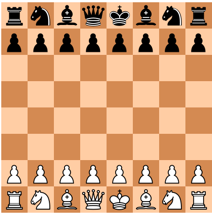
\includegraphics[width=\linewidth]{chess1}
  \caption{Starting position}\label{fig:chess1}
\endminipage\hfill
\minipage{0.32\textwidth}%
  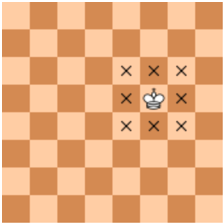
\includegraphics[width=\linewidth]{chess2}
  \caption{King}\label{fig:chess2}
\endminipage\hfill
\minipage{0.32\textwidth}%
  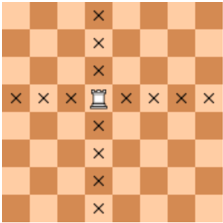
\includegraphics[width=\linewidth]{chess3}
  \caption{Rook}\label{fig:chess3}
\endminipage
\end{figure}
\begin{figure}[!htb]
\minipage{0.32\textwidth}%
  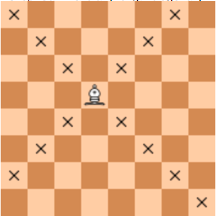
\includegraphics[width=\linewidth]{chess4}
  \caption{Bishop}\label{fig:chess4}
\endminipage\hfill
\minipage{0.32\textwidth}%
  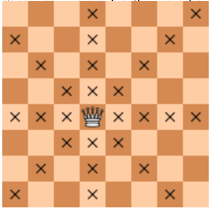
\includegraphics[width=\linewidth]{chess5}
  \caption{Queen}\label{fig:chess5}
\endminipage\hfill
\minipage{0.32\textwidth}%
  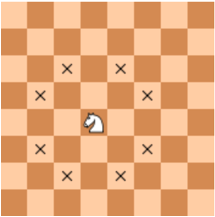
\includegraphics[width=\linewidth]{chess6}
  \caption{Knight}\label{fig:chess6}
\endminipage
\end{figure}

\subsection*{Capturing}

Pieces can capture enemy pieces in order to remove them from the board. Capturing works by moving a piece onto the square of an enemy piece - the enemy piece is then removed from the game. A player cannot capture their own pieces. Normally, a piece can only capture pieces on positions they could have moved to if the position was empty. Capturing a piece ends the player's turn, and the moved piece may go no further.\\

\noindent
Exceptions:

\begin{easylist}[itemize]
# The king cannot capture a piece if this puts him in a threatened position.
# The pawn cannot capture pieces my moving forward, but instead capture by moving one step diagonally forward and to the left or right.
\end{easylist}

\subsection*{Game over}

The game can be won by either white or black, or can result in a draw if specific conditions are met.

\subsubsection*{Check and checkmate}

The game is played with the intention of putting the other player in \textbf{checkmate}. A player is in checkmate if their king is threatened by an enemy piece and has no legal moves. If a player is in checkmate, the other player wins the game.

A lesser version of checkmate is \textbf{check}. A player is in check if their king is threatened, but they have legal moves to perform that result in the king not being threatened anymore. If this situation occurs, the player \textit{must} perform one of these moves.

\subsubsection*{Other win/loss conditions}

A player may also \textbf{resign} if they see no hope of winning the game. In this situation, the opponent player also wins the game. In versions of the game where the duration of player turns are time-constrained, a player also loses if their \textbf{time runs out} before they have made a move and ended their turn.

\subsubsection*{Draws}

The game can result in a draw for several reasons:\\

\noindent
\textbf{Stalemate:} The player is not in check, but there are no legal moves (as any attempt to perform a move would put the king in check).\\


\noindent
\textbf{Insufficient material:} There are not enough pieces remaining for checkmate to occur. This is the case when the board contains:

\begin{easylist}[itemize]
# King vs. king
# King vs. king and bishop
# King vs. king and knight
# King and bishop vs. king and bishop, if both the bishops occupy the same colored square
\end{easylist}\mbox{}\\

\noindent
\textbf{Player agreement:} If both players agree to a draw, the game is drawn.\\

\noindent
\textbf{Fifty-move rule:} A player can claim a draw by declaring that there has been no capture or pawn move in the last fifty moves, if their claim is proven true.\\

\noindent
\textbf{Threefold repetition:} A player can claim a draw by declaring that the same board position has occurred three times on the turn of the same player where their pieces have the same possible moves (including castling and en passant), if their claim is proven true.

\newpage
\subsection*{Special moves}
\textbf{Castling:} This is a move that can be performed at most once per player, once per game. It's the only move which changes the position of two pieces, a king and one of the rooks. It requires that neither the king nor the rook has previously moved and are in their starting positions. Furthermore, it requires that the king is not in check, and will not pass over any squares threatened by an enemy piece, and that there are no pieces between the king and the rook. The king moves two steps towards the rook, and the castle is placed on the other side of the king, next to the king's original position. See figure 7 and 8. \\

\noindent
\textbf{En passant:} If the opponents pawn moves two steps forward from the starting position, and is thus placed next to your own pawn, you are allowed to strike it as if it had only moved one step forward. See figure 9 and 10.\\

\noindent
\textbf{Promotion:} A pawn piece reaching the far end of the board is replaced with a queen piece.

\begin{figure}[!htb]
\minipage{0.32\textwidth}%
    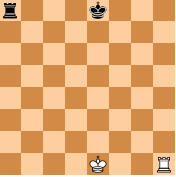
\includegraphics[width=\linewidth]{before-castling}
    \caption{Before castling}\label{fig:chess7}
\endminipage\hfill
\minipage{0.32\textwidth}%
    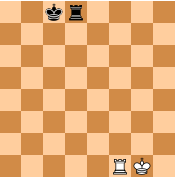
\includegraphics[width=\linewidth]{after-castling}
    \caption{After castling}\label{fig:chess9}
\endminipage\hfill
\end{figure}
\begin{figure}[!htb]
\minipage{0.32\textwidth}%
    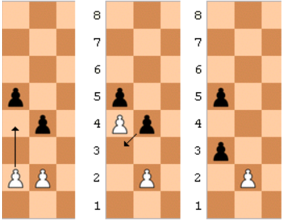
\includegraphics[width=\linewidth]{chess10}
    \caption{En passant}\label{fig:chess8}
\endminipage
\end{figure}

\section*{Sjadam}
\subsection*{Basics}

Sjadam is similar to normal chess which consist a chess board and 32 pieces, 16 black and 16 white. The board still consist of 8x8 squares with all original pieces from normal chess. The game is turn based where player can perform a move each turn. The different is player can now perform sjadam jump which is an extra move. White always goes first. Rules, conditions are the same as regular chess with a few exceptions . 

\subsection*{Sjadam jump}

Player may start the move with either a sjadam jump or a legal chess move. The sjadam jump is only valid if player can jump over a piece onto an empty field and it can be in any direction. You can jump over as many of your own pieces as you like, but only over one opponent piece each turn.

\subsection*{promotion}

In regular chess, there is only pawn can be promoted to a queen when the piece is all the way onto the other side of the board. In sjadam chess, any piece except the king can be promoted to a queen. 


\section*{Firechess}
\subsection*{Basics}

Our game is based on a hand drawn theme, and we tried to make it as reslistic as possible. The idea of this game mode is to burn the board while playing. The game rules are just like regular chess with a limited time as the board is being burn slowly,it takes approximately 10 minutes for the flame to reach the centre of the board for each player. The game consist a chess 8x8 squares with 32 pieces, 16 black and 16 white. It is still a turn based game with white always goes first. 


\subsection*{Capturing and burned pieces}

Pieces can capture enemy pieces in order to remove them from the board. If the fire touches a piece there will be a water splash which drives the fire away a bit and the piece that is touched is then removed from the game. A player cannot capture their own pieces but they can sacrifice pieces to make the water splash away the fire. The water splash is circlular. There are 6 types of pieces in chess and each of them have different sized water splash. The size of water splash is proportional to the size of the piece point. 

\subsection*{Legal move}

Piece cannot be move onto burned area. 




 



\end{document}
